\documentclass{book}
\usepackage[a4paper,top=2.5cm,bottom=2.5cm,left=2.5cm,right=2.5cm]{geometry}
\usepackage{makeidx}
\usepackage{natbib}
\usepackage{graphicx}
\usepackage{multicol}
\usepackage{float}
\usepackage{listings}
\usepackage{color}
\usepackage{ifthen}
\usepackage[table]{xcolor}
\usepackage{textcomp}
\usepackage{alltt}
\usepackage[utf8]{inputenc}
\usepackage{mathptmx}
\usepackage[scaled=.90]{helvet}
\usepackage{courier}
\usepackage{sectsty}
\usepackage{amssymb}
\usepackage[titles]{tocloft}
\usepackage{doxygen}
\lstset{language=C++,inputencoding=utf8,basicstyle=\footnotesize,breaklines=true,breakatwhitespace=true,tabsize=8,numbers=left }
\makeindex
\setcounter{tocdepth}{3}
\renewcommand{\footrulewidth}{0.4pt}
\renewcommand{\familydefault}{\sfdefault}
\hfuzz=15pt
\setlength{\emergencystretch}{15pt}
\hbadness=750
\tolerance=750
\begin{document}
\begin{titlepage}
\vspace*{7cm}
\begin{center}
{\Large Trivent \\[1ex]\large 0.\-4.\-2 }\\
\vspace*{1cm}
{\large Generated by Doxygen 1.8.3.1}\\
\vspace*{0.5cm}
{\small Wed Aug 7 2013 19:55:52}\\
\end{center}
\end{titlepage}
\clearemptydoublepage
\pagenumbering{roman}
\tableofcontents
\clearemptydoublepage
\pagenumbering{arabic}
\chapter{Hierarchical Index}
\section{Class Hierarchy}
This inheritance list is sorted roughly, but not completely, alphabetically\-:\begin{DoxyCompactList}
\item \contentsline{section}{Coll\-Tree}{\pageref{classCollTree}}{}
\item \contentsline{section}{D\-I\-F\-Ptr}{\pageref{classDIFPtr}}{}
\item \contentsline{section}{D\-I\-F\-Slow\-Control}{\pageref{classDIFSlowControl}}{}
\item \contentsline{section}{D\-I\-F\-Unpacker}{\pageref{classDIFUnpacker}}{}
\item \contentsline{section}{Gain\-Correct}{\pageref{classGainCorrect}}{}
\item \contentsline{section}{Gain\-Hist}{\pageref{structGainHist}}{}
\item \contentsline{section}{Hist\-Def\-T\-H1\-F}{\pageref{classHistDefTH1F}}{}
\item \contentsline{section}{Hist\-Def\-T\-H2\-F}{\pageref{classHistDefTH2F}}{}
\item \contentsline{section}{Hist\-Def\-T\-Prof}{\pageref{classHistDefTProf}}{}
\item \contentsline{section}{Layer\-I\-D}{\pageref{structLayerID}}{}
\item L\-C\-Generic\-Object\-Impl\begin{DoxyCompactList}
\item \contentsline{section}{L\-M\-Generic}{\pageref{classLMGeneric}}{}
\end{DoxyCompactList}
\item pair\begin{DoxyCompactList}
\item \contentsline{section}{S\-D\-H\-C\-A\-L\-\_\-buffer}{\pageref{classSDHCAL__buffer}}{}
\end{DoxyCompactList}
\item Processor\begin{DoxyCompactList}
\item \contentsline{section}{Trivent\-Proc}{\pageref{classTriventProc}}{}
\end{DoxyCompactList}
\item Processor\begin{DoxyCompactList}
\item \contentsline{section}{S\-D\-H\-C\-A\-L\-\_\-\-Raw\-Data\-\_\-\-Processor}{\pageref{classSDHCAL__RawData__Processor}}{}
\end{DoxyCompactList}
\item \contentsline{section}{S\-D\-H\-C\-A\-L\-\_\-\-Raw\-Buffer\-\_\-\-Navigator}{\pageref{classSDHCAL__RawBuffer__Navigator}}{}
\end{DoxyCompactList}

\chapter{Class Index}
\section{Class List}
Here are the classes, structs, unions and interfaces with brief descriptions\-:\begin{DoxyCompactList}
\item\contentsline{section}{{\bf Coll\-Tree} }{\pageref{classCollTree}}{}
\item\contentsline{section}{{\bf D\-I\-F\-Ptr} }{\pageref{classDIFPtr}}{}
\item\contentsline{section}{{\bf D\-I\-F\-Slow\-Control} \\*Handler of D\-I\-F Slow Control info }{\pageref{classDIFSlowControl}}{}
\item\contentsline{section}{{\bf D\-I\-F\-Unpacker} }{\pageref{classDIFUnpacker}}{}
\item\contentsline{section}{{\bf Gain\-Correct} }{\pageref{classGainCorrect}}{}
\item\contentsline{section}{{\bf Gain\-Hist} }{\pageref{structGainHist}}{}
\item\contentsline{section}{{\bf Hist\-Def\-T\-H1\-F} }{\pageref{classHistDefTH1F}}{}
\item\contentsline{section}{{\bf Hist\-Def\-T\-H2\-F} }{\pageref{classHistDefTH2F}}{}
\item\contentsline{section}{{\bf Hist\-Def\-T\-Prof} }{\pageref{classHistDefTProf}}{}
\item\contentsline{section}{{\bf Layer\-I\-D} }{\pageref{structLayerID}}{}
\item\contentsline{section}{{\bf L\-M\-Generic} }{\pageref{classLMGeneric}}{}
\item\contentsline{section}{{\bf S\-D\-H\-C\-A\-L\-\_\-buffer} }{\pageref{classSDHCAL__buffer}}{}
\item\contentsline{section}{{\bf S\-D\-H\-C\-A\-L\-\_\-\-Raw\-Buffer\-\_\-\-Navigator} }{\pageref{classSDHCAL__RawBuffer__Navigator}}{}
\item\contentsline{section}{{\bf S\-D\-H\-C\-A\-L\-\_\-\-Raw\-Data\-\_\-\-Processor} }{\pageref{classSDHCAL__RawData__Processor}}{}
\item\contentsline{section}{{\bf Trivent\-Proc} }{\pageref{classTriventProc}}{}
\end{DoxyCompactList}

\chapter{Class Documentation}
\section{Coll\-Tree Class Reference}
\label{classCollTree}\index{Coll\-Tree@{Coll\-Tree}}


\subsection{Detailed Description}


Definition at line 61 of file Histogram\-Hendler.\-h.



The documentation for this class was generated from the following files\-:\begin{DoxyCompactItemize}
\item 
Histogram\-Hendler.\-h\item 
Histogram\-Handler.\-cc\end{DoxyCompactItemize}

\section{D\-I\-F\-Ptr Class Reference}
\label{classDIFPtr}\index{D\-I\-F\-Ptr@{D\-I\-F\-Ptr}}
\subsection*{Public Member Functions}
\begin{DoxyCompactItemize}
\item 
{\bfseries D\-I\-F\-Ptr} (unsigned char $\ast$p, uint32\-\_\-t max\-\_\-size)\label{classDIFPtr_a1ec95322a11ec222592d69d947003067}

\item 
unsigned char $\ast$ {\bfseries get\-Ptr} ()\label{classDIFPtr_ad651990bff2ceda40ef902a881aeeec0}

\item 
uint32\-\_\-t {\bfseries get\-Get\-Frame\-Ptr\-Return} ()\label{classDIFPtr_a2c2a47771ad37cadbeea63c4dc987a74}

\item 
std\-::vector$<$ unsigned char $\ast$ $>$ \& {\bfseries get\-Frames\-Vector} ()\label{classDIFPtr_aa866203b824bc6127101ecc49f140deb}

\item 
std\-::vector$<$ unsigned char $\ast$ $>$ \& {\bfseries get\-Lines\-Vector} ()\label{classDIFPtr_ac3eabe969d84da39c5b3f1b02d6b2d50}

\item 
uint32\-\_\-t {\bfseries get\-I\-D} ()\label{classDIFPtr_a86a54006ce18b2edb5f94122cd46258f}

\item 
uint32\-\_\-t {\bfseries get\-D\-T\-C} ()\label{classDIFPtr_a185ff7c335f92dbbf419a20f12f23982}

\item 
uint32\-\_\-t {\bfseries get\-G\-T\-C} ()\label{classDIFPtr_ab907406b86a9208546ee80e2853752a9}

\item 
unsigned long long {\bfseries get\-Absolute\-B\-C\-I\-D} ()\label{classDIFPtr_a6bef56775da90f86385ce87f168a1fc7}

\item 
uint32\-\_\-t {\bfseries get\-B\-C\-I\-D} ()\label{classDIFPtr_a595f75322176a9a1fda707aefc5b5f9b}

\item 
uint32\-\_\-t {\bfseries get\-Lines} ()\label{classDIFPtr_af77cccc02ff318f5ef57c1cc59e63e3c}

\item 
bool {\bfseries has\-Line} (uint32\-\_\-t line)\label{classDIFPtr_a02a04813a664f59ae62c18e7028e1492}

\item 
uint32\-\_\-t {\bfseries get\-T\-A\-S\-U1} ()\label{classDIFPtr_a71bf41db6c238b918d77f31e6cafd8f0}

\item 
uint32\-\_\-t {\bfseries get\-T\-A\-S\-U2} ()\label{classDIFPtr_abcf41a39b0b0b30d0eb2029a38259eb8}

\item 
uint32\-\_\-t {\bfseries get\-T\-D\-I\-F} ()\label{classDIFPtr_a439b05313396e5278faf6bb8a20b0d36}

\item 
float {\bfseries get\-Temperature\-D\-I\-F} ()\label{classDIFPtr_af3aee586fadb7fc6c606d943fb46c06f}

\item 
float {\bfseries get\-Temperature\-A\-S\-U1} ()\label{classDIFPtr_a9b80907d5204fa2cd67edcd6e5bfcffe}

\item 
float {\bfseries get\-Temperature\-A\-S\-U2} ()\label{classDIFPtr_acb4e874dbd731ed2ffaa30c8c12f9e04}

\item 
bool {\bfseries has\-Temperature} ()\label{classDIFPtr_ac610d35950f4b116a7ed4ef5655bcddf}

\item 
bool {\bfseries has\-Analog\-Readout} ()\label{classDIFPtr_a5d02923a395f2a7a97eae4c6b9653773}

\item 
uint32\-\_\-t {\bfseries get\-Number\-Of\-Frames} ()\label{classDIFPtr_a16798cd9a47f3e4358af1fd3ba390164}

\item 
unsigned char $\ast$ {\bfseries get\-Frame\-Ptr} (uint32\-\_\-t i)\label{classDIFPtr_a33da5d922051cec1b9823764b0588d2f}

\item 
uint32\-\_\-t {\bfseries get\-Frame\-Asic\-Header} (uint32\-\_\-t i)\label{classDIFPtr_a4645862d450eaf77011d3425dc841978}

\item 
uint32\-\_\-t {\bfseries get\-Frame\-B\-C\-I\-D} (uint32\-\_\-t i)\label{classDIFPtr_a3ce47db6d214f1e99b97fbb625d248d3}

\item 
uint32\-\_\-t {\bfseries get\-Frame\-Time\-To\-Trigger} (uint32\-\_\-t i)\label{classDIFPtr_a9ca659e4ec65e127990be939f36a73f5}

\item 
bool {\bfseries get\-Frame\-Level} (uint32\-\_\-t i, uint32\-\_\-t ipad, uint32\-\_\-t ilevel)\label{classDIFPtr_af97896aadd544502d319846073c319e0}

\item 
void {\bfseries dump\-D\-I\-F\-Info} ()\label{classDIFPtr_a949bb0b6ac03ddb99c7ec73bd6699ec9}

\end{DoxyCompactItemize}


\subsection{Detailed Description}


Definition at line 77 of file D\-I\-F\-Slow\-Control.\-h.



The documentation for this class was generated from the following file\-:\begin{DoxyCompactItemize}
\item 
D\-I\-F\-Slow\-Control.\-h\end{DoxyCompactItemize}

\section{D\-I\-F\-Slow\-Control Class Reference}
\label{classDIFSlowControl}\index{D\-I\-F\-Slow\-Control@{D\-I\-F\-Slow\-Control}}


Handler of D\-I\-F Slow Control info.  




{\ttfamily \#include $<$D\-I\-F\-Slow\-Control.\-h$>$}

\subsection*{Public Member Functions}
\begin{DoxyCompactItemize}
\item 
{\bf D\-I\-F\-Slow\-Control} (unsigned int version, unsigned short D\-Idi, unsigned char $\ast$buf)
\begin{DoxyCompactList}\small\item\em Constructor. \end{DoxyCompactList}\item 
{\bf D\-I\-F\-Slow\-Control} ()\label{classDIFSlowControl_a9ab99ff41ff746c990ca475d6edb4158}

\begin{DoxyCompactList}\small\item\em Default Cosntructor. \end{DoxyCompactList}\item 
unsigned short {\bf get\-D\-I\-F\-Id} ()\label{classDIFSlowControl_aa9709f45bc7dd629013f850ac8d3ef55}

\begin{DoxyCompactList}\small\item\em get D\-I\-F id \end{DoxyCompactList}\item 
map$<$ int, map$<$ string, int $>$ $>$ {\bf get\-Chips\-Map} ()
\begin{DoxyCompactList}\small\item\em Get chips map. \end{DoxyCompactList}\item 
map$<$ string, int $>$ {\bf get\-Chip\-Slow\-Control} (int asicid)
\begin{DoxyCompactList}\small\item\em Get one chip map. \end{DoxyCompactList}\item 
int {\bf get\-Chip\-Slow\-Control} (int asicid, string param)
\begin{DoxyCompactList}\small\item\em Get one Chip value. \end{DoxyCompactList}\item 
void {\bf Dump} ()\label{classDIFSlowControl_af5d12af4062366925fbe631687f987dd}

\begin{DoxyCompactList}\small\item\em print out full map \end{DoxyCompactList}\end{DoxyCompactItemize}


\subsection{Detailed Description}
Handler of D\-I\-F Slow Control info. 

\begin{DoxyAuthor}{Author}
L.\-Mirabito 
\end{DoxyAuthor}
\begin{DoxyDate}{Date}
March 2010 
\end{DoxyDate}
\begin{DoxyVersion}{Version}
1.\-0 
\end{DoxyVersion}


Definition at line 20 of file D\-I\-F\-Slow\-Control.\-h.



\subsection{Constructor \& Destructor Documentation}
\index{D\-I\-F\-Slow\-Control@{D\-I\-F\-Slow\-Control}!D\-I\-F\-Slow\-Control@{D\-I\-F\-Slow\-Control}}
\index{D\-I\-F\-Slow\-Control@{D\-I\-F\-Slow\-Control}!DIFSlowControl@{D\-I\-F\-Slow\-Control}}
\subsubsection[{D\-I\-F\-Slow\-Control}]{\setlength{\rightskip}{0pt plus 5cm}D\-I\-F\-Slow\-Control\-::\-D\-I\-F\-Slow\-Control (
\begin{DoxyParamCaption}
\item[{unsigned int}]{version, }
\item[{unsigned short}]{D\-Idi, }
\item[{unsigned char $\ast$}]{buf}
\end{DoxyParamCaption}
)}\label{classDIFSlowControl_a7c579de8938c49d0ad78c31edb6e8198}


Constructor. 


\begin{DoxyParams}{Parameters}
{\em version} & Data format version \\
\hline
{\em D\-Idi} & D\-I\-F id \\
\hline
{\em buf} & Pointer to the Raw data buffer \\
\hline
\end{DoxyParams}


Definition at line 59 of file D\-I\-F\-Slow\-Control.\-cc.


\begin{DoxyCode}
60 \{
61   \_DIFId=DIdi;
62   \_version=vers;
63   \_asicType=2;
64   \textcolor{comment}{// }
65   \textcolor{comment}{//std::cout<<"DIFSlowControl :: "<<std::hex<<(int)cbuf[0]<<std::dec<<std::endl;}
66   \textcolor{keywordflow}{if} (cbuf[0]!=0xb1) \textcolor{keywordflow}{return};
67   \textcolor{keywordtype}{int} header\_shift=6;
68   \textcolor{keywordflow}{if} (\_version<8) 
69     \_nAsic=cbuf[5];
70   \textcolor{keywordflow}{else}
71     \{
72       \_DIFId=cbuf[1];
73       \_nAsic= cbuf[2];
74       header\_shift=3;
75     \}
76 
77   \textcolor{comment}{//std::cout<<" Id version header shift "<<\_DIFId<<" "<<\_version<<" "<<\_nAsic<<"
       "<<header\_shift<<std::endl;}
78   \textcolor{keywordtype}{int} size\_hardroc1 = \_nAsic*72+header\_shift+1;
79   \textcolor{keywordflow}{if} (cbuf[size\_hardroc1-1]!=0xa1) size\_hardroc1=0;
80 
81   \textcolor{keywordtype}{int} size\_hardroc2 = \_nAsic*109+header\_shift+1;
82   \textcolor{keywordflow}{if} (cbuf[size\_hardroc2-1]!=0xa1) size\_hardroc2=0;
83   
84   \textcolor{comment}{//std::cout<<" Hardroc 1 "<<size\_hardroc1<<" "<<(int)cbuf[size\_hardroc1-1]<<" "<<(int)
       cbuf[size\_hardroc1]<<std::endl;}
85   \textcolor{comment}{//std::cout<<" Hardroc 2 "<<size\_hardroc2<<" "<<(int)cbuf[size\_hardroc2-1]<<" "<<(int)
       cbuf[size\_hardroc2]<<std::endl;}
86 
87   \textcolor{keywordflow}{if} (size\_hardroc1!=0)
88     \{
89     FillHR1(header\_shift,cbuf);
90     \_asicType=1;
91     \}
92   \textcolor{keywordflow}{else}
93     \textcolor{keywordflow}{if} (size\_hardroc2!=0)
94       FillHR2(header\_shift,cbuf);
95     \textcolor{keywordflow}{else}
96       \textcolor{keywordflow}{return};
97 
98 
99 
100 
101   
102 \}
\end{DoxyCode}


\subsection{Member Function Documentation}
\index{D\-I\-F\-Slow\-Control@{D\-I\-F\-Slow\-Control}!get\-Chip\-Slow\-Control@{get\-Chip\-Slow\-Control}}
\index{get\-Chip\-Slow\-Control@{get\-Chip\-Slow\-Control}!DIFSlowControl@{D\-I\-F\-Slow\-Control}}
\subsubsection[{get\-Chip\-Slow\-Control}]{\setlength{\rightskip}{0pt plus 5cm}map$<$string,int$>$ D\-I\-F\-Slow\-Control\-::get\-Chip\-Slow\-Control (
\begin{DoxyParamCaption}
\item[{int}]{asicid}
\end{DoxyParamCaption}
)\hspace{0.3cm}{\ttfamily [inline]}}\label{classDIFSlowControl_ad37d6fe51915ee489ff7b026abb48c24}


Get one chip map. 


\begin{DoxyParams}{Parameters}
{\em asicid} & A\-S\-I\-C I\-D \\
\hline
\end{DoxyParams}
\begin{DoxyReturn}{Returns}
a map of $<$string (parameter name),int (parameter value) $>$ 
\end{DoxyReturn}


Definition at line 47 of file D\-I\-F\-Slow\-Control.\-h.


\begin{DoxyCode}
47 \{ \textcolor{keywordflow}{return} \_mapSC[asicid];\}
\end{DoxyCode}
\index{D\-I\-F\-Slow\-Control@{D\-I\-F\-Slow\-Control}!get\-Chip\-Slow\-Control@{get\-Chip\-Slow\-Control}}
\index{get\-Chip\-Slow\-Control@{get\-Chip\-Slow\-Control}!DIFSlowControl@{D\-I\-F\-Slow\-Control}}
\subsubsection[{get\-Chip\-Slow\-Control}]{\setlength{\rightskip}{0pt plus 5cm}int D\-I\-F\-Slow\-Control\-::get\-Chip\-Slow\-Control (
\begin{DoxyParamCaption}
\item[{int}]{asicid, }
\item[{string}]{param}
\end{DoxyParamCaption}
)\hspace{0.3cm}{\ttfamily [inline]}}\label{classDIFSlowControl_a5a3958416420d777f57f6c5b45467a9a}


Get one Chip value. 


\begin{DoxyParams}{Parameters}
{\em asicid} & A\-Sic I\-D \\
\hline
{\em param} & Parameter name \\
\hline
\end{DoxyParams}


Definition at line 54 of file D\-I\-F\-Slow\-Control.\-h.



References get\-Chip\-Slow\-Control().



Referenced by get\-Chip\-Slow\-Control().


\begin{DoxyCode}
54 \{ \textcolor{keywordflow}{return} getChipSlowControl(asicid)[param];\}
\end{DoxyCode}
\index{D\-I\-F\-Slow\-Control@{D\-I\-F\-Slow\-Control}!get\-Chips\-Map@{get\-Chips\-Map}}
\index{get\-Chips\-Map@{get\-Chips\-Map}!DIFSlowControl@{D\-I\-F\-Slow\-Control}}
\subsubsection[{get\-Chips\-Map}]{\setlength{\rightskip}{0pt plus 5cm}map$<$ int,map $<$string,int$>$ $>$ D\-I\-F\-Slow\-Control\-::get\-Chips\-Map (
\begin{DoxyParamCaption}
{}
\end{DoxyParamCaption}
)\hspace{0.3cm}{\ttfamily [inline]}}\label{classDIFSlowControl_a58644b35bd873ac0f104c2b59825020c}


Get chips map. 

\begin{DoxyReturn}{Returns}
a map of $<$ Asic Id, map of $<$string (parameter name),int (parameter value) $>$ 
\end{DoxyReturn}


Definition at line 40 of file D\-I\-F\-Slow\-Control.\-h.


\begin{DoxyCode}
40 \{ \textcolor{keywordflow}{return} \_mapSC;\}
\end{DoxyCode}


The documentation for this class was generated from the following files\-:\begin{DoxyCompactItemize}
\item 
D\-I\-F\-Slow\-Control.\-h\item 
D\-I\-F\-Slow\-Control.\-cc\end{DoxyCompactItemize}

\section{D\-I\-F\-Unpacker Class Reference}
\label{classDIFUnpacker}\index{D\-I\-F\-Unpacker@{D\-I\-F\-Unpacker}}
\subsection*{Static Public Member Functions}
\begin{DoxyCompactItemize}
\item 
static unsigned long long {\bfseries Gray\-To\-Bin} (unsigned long long n)\label{classDIFUnpacker_ac74ff0751283b47ec3305e6bd097f205}

\item 
static uint32\-\_\-t {\bfseries get\-Start\-Of\-D\-I\-F} (unsigned char $\ast$cbuf, uint32\-\_\-t size\-\_\-buf, uint32\-\_\-t start=92)\label{classDIFUnpacker_a86b0d092ea83532cff54ab8ef84e6a4d}

\item 
static uint32\-\_\-t {\bfseries get\-I\-D} (unsigned char $\ast$cb, uint32\-\_\-t idx=0)\label{classDIFUnpacker_a4b106d75d0bbe55aaa04543b803c570c}

\item 
static uint32\-\_\-t {\bfseries get\-D\-T\-C} (unsigned char $\ast$cb, uint32\-\_\-t idx=0)\label{classDIFUnpacker_a386f40719e54da21a043aaaa2f99a923}

\item 
static uint32\-\_\-t {\bfseries get\-G\-T\-C} (unsigned char $\ast$cb, uint32\-\_\-t idx=0)\label{classDIFUnpacker_a1c394b50668906c62aa4ffceb17afa64}

\item 
static unsigned long long {\bfseries get\-Absolute\-B\-C\-I\-D} (unsigned char $\ast$cb, uint32\-\_\-t idx=0)\label{classDIFUnpacker_a74793ca664243ae4c8a0208429e4f616}

\item 
static uint32\-\_\-t {\bfseries get\-B\-C\-I\-D} (unsigned char $\ast$cb, uint32\-\_\-t idx=0)\label{classDIFUnpacker_ac76f67110c4bedc0c61aaf8debc40733}

\item 
static uint32\-\_\-t {\bfseries get\-Lines} (unsigned char $\ast$cb, uint32\-\_\-t idx=0)\label{classDIFUnpacker_a2758864b517c88fe23a63d0d4e42ea03}

\item 
static bool {\bfseries has\-Line} (uint32\-\_\-t line, unsigned char $\ast$cb, uint32\-\_\-t idx=0)\label{classDIFUnpacker_aa0bb59ee85f241b4f5e05600315fe2ab}

\item 
static uint32\-\_\-t {\bfseries get\-T\-A\-S\-U1} (unsigned char $\ast$cb, uint32\-\_\-t idx=0)\label{classDIFUnpacker_a53856c28021d5fb4e6456971f982eb18}

\item 
static uint32\-\_\-t {\bfseries get\-T\-A\-S\-U2} (unsigned char $\ast$cb, uint32\-\_\-t idx=0)\label{classDIFUnpacker_ae0637a6a2f2f125e32fa61bc01bd17f2}

\item 
static uint32\-\_\-t {\bfseries get\-T\-D\-I\-F} (unsigned char $\ast$cb, uint32\-\_\-t idx=0)\label{classDIFUnpacker_a6d9a18d21dafac9dacc738d623b7e882}

\item 
static bool {\bfseries has\-Temperature} (unsigned char $\ast$cb, uint32\-\_\-t idx=0)\label{classDIFUnpacker_a0a70ac9ebc523e4289088967f2e518c5}

\item 
static bool {\bfseries has\-Analog\-Readout} (unsigned char $\ast$cb, uint32\-\_\-t idx=0)\label{classDIFUnpacker_aa02d8c21418823e1fa9fe0364e21a13d}

\item 
static uint32\-\_\-t {\bfseries get\-Frame\-Asic\-Header} (unsigned char $\ast$frame\-Ptr)\label{classDIFUnpacker_ae9004570d90ff565d8b18aa96222d4bc}

\item 
static uint32\-\_\-t {\bfseries get\-Frame\-B\-C\-I\-D} (unsigned char $\ast$frame\-Ptr)\label{classDIFUnpacker_a2ac77487a6292a01969859e8546f63de}

\item 
static bool {\bfseries get\-Frame\-P\-A\-D} (unsigned char $\ast$frame\-Ptr, uint32\-\_\-t ip)\label{classDIFUnpacker_a7dcd946045bfd90eacc02febd81237f1}

\item 
static bool {\bfseries get\-Frame\-Level} (unsigned char $\ast$frame\-Ptr, uint32\-\_\-t ip, uint32\-\_\-t level)\label{classDIFUnpacker_ae9dd6ecdd0a26d8c0b3dfe5407733d0a}

\item 
static uint32\-\_\-t {\bfseries get\-Analog\-Ptr} (std\-::vector$<$ unsigned char $\ast$ $>$ \&v\-Lines, unsigned char $\ast$cb, uint32\-\_\-t idx=0)  throw (std\-::string)\label{classDIFUnpacker_a17e12f0a800b6b9b1fa39f5ecf83d7c5}

\item 
static uint32\-\_\-t {\bfseries get\-Frame\-Ptr} (std\-::vector$<$ unsigned char $\ast$ $>$ \&v\-Frame, std\-::vector$<$ unsigned char $\ast$ $>$ \&v\-Lines, uint32\-\_\-t max\-\_\-size, unsigned char $\ast$cb, uint32\-\_\-t idx=0)  throw (std\-::string)\label{classDIFUnpacker_a5ab111b5d6acdeefd29648199800f27e}

\item 
static void {\bfseries dump\-Frame\-Old} (unsigned char $\ast$buf)\label{classDIFUnpacker_a24d530b0a8f9c525b9e1f569fd7e800f}

\item 
static unsigned long {\bfseries swap\-\_\-bytes} (unsigned int n, unsigned char $\ast$buf)\label{classDIFUnpacker_ab0b206c3dde528aca2b5d098b6314952}

\end{DoxyCompactItemize}


\subsection{Detailed Description}


Definition at line 34 of file D\-I\-F\-Unpacker.\-h.



The documentation for this class was generated from the following files\-:\begin{DoxyCompactItemize}
\item 
D\-I\-F\-Unpacker.\-h\item 
D\-I\-F\-Unpacker.\-cc\end{DoxyCompactItemize}

\section{Gain\-Correct Class Reference}
\label{classGainCorrect}\index{Gain\-Correct@{Gain\-Correct}}
\subsection*{Public Member Functions}
\begin{DoxyCompactItemize}
\item 
uint {\bfseries get\-Cell\-Dif\-\_\-id} (int cell\-\_\-id)\label{classGainCorrect_a0f6582bebdcb7c7e28a50b976b516889}

\item 
uint {\bfseries get\-Cell\-Asic\-\_\-id} (int cell\-\_\-id)\label{classGainCorrect_ad47b491a5cfc05d302bcfe89355139dc}

\item 
uint {\bfseries get\-Cell\-Chan\-\_\-id} (int cell\-\_\-id)\label{classGainCorrect_aadd9201c4bb5477ebd8c844c470870c5}

\item 
void {\bfseries gain\-Correction\-Init} (std\-::map$<$ int, {\bf Layer\-I\-D} $>$ \-\_\-mapping)\label{classGainCorrect_a9d22fc0d5f046f1a97b7924e76b0aeb3}

\item 
void {\bfseries gain\-Correction\-Parser} (E\-V\-E\-N\-T\-::\-L\-C\-Collection $\ast$col)\label{classGainCorrect_a6d1f995946c98bbe9320de624b57e32e}

\item 
void {\bfseries gain\-Corrector} (const string gain\-\_\-file)\label{classGainCorrect_a437c2fccc62f1ecf676f3fd2e510fa54}

\end{DoxyCompactItemize}
\subsection*{Protected Attributes}
\begin{DoxyCompactItemize}
\item 
std\-::map$<$ int, {\bf Layer\-I\-D} $>$ {\bfseries \-\_\-mapping}\label{classGainCorrect_aff3835d1b24e6a6a7bfaa4d10158e13d}

\item 
std\-::map$<$ int, {\bf Gain\-Hist} $>$ {\bfseries \-\_\-h\-\_\-gain}\label{classGainCorrect_a67c3261e2ee9c65aa617661ef634052c}

\item 
T\-H1\-F $\ast$ {\bfseries noise\-\_\-dist}\label{classGainCorrect_a923de2eb0f07ab046e8c0205ac1ff968}

\item 
T\-H1\-F $\ast$ {\bfseries gain\-\_\-chan}\label{classGainCorrect_a38da4f5cc568c29f328cc09a1d780b7f}

\item 
T\-H1\-F $\ast$ {\bfseries mean\-\_\-hit\-\_\-dif}\label{classGainCorrect_aae8b02a5da778ef4fb29ad4b1d672d6a}

\item 
T\-H1\-F $\ast$ {\bfseries time\-\_\-hit\-\_\-dif}\label{classGainCorrect_ac468b93238fcf95b7d5d32c5a6724875}

\end{DoxyCompactItemize}


\subsection{Detailed Description}


Definition at line 23 of file Gain\-Correct.\-h.



The documentation for this class was generated from the following files\-:\begin{DoxyCompactItemize}
\item 
Gain\-Correct.\-h\item 
Gain\-Correct.\-cc\end{DoxyCompactItemize}

\section{Gain\-Hist Struct Reference}
\label{structGainHist}\index{Gain\-Hist@{Gain\-Hist}}
\subsection*{Public Attributes}
\begin{DoxyCompactItemize}
\item 
T\-H1\-F $\ast$ {\bfseries noise\-\_\-on\-\_\-dif}\label{structGainHist_a3f4b2c4b6da381be1639bcf91e1b09ec}

\item 
T\-H1\-F $\ast$ {\bfseries gain\-\_\-chan}\label{structGainHist_a672b31f0e7a6fd8aeb98e22d810018a1}

\end{DoxyCompactItemize}


\subsection{Detailed Description}


Definition at line 18 of file Gain\-Correct.\-h.



The documentation for this struct was generated from the following file\-:\begin{DoxyCompactItemize}
\item 
Gain\-Correct.\-h\end{DoxyCompactItemize}

\section{Hist\-Def\-T\-H1\-F Class Reference}
\label{classHistDefTH1F}\index{Hist\-Def\-T\-H1\-F@{Hist\-Def\-T\-H1\-F}}
\subsection*{Public Attributes}
\begin{DoxyCompactItemize}
\item 
Text\-\_\-t $\ast$ {\bfseries name}\label{classHistDefTH1F_ab1da75ca62e61ac7e8b08228be812a3e}

\item 
Text\-\_\-t $\ast$ {\bfseries title}\label{classHistDefTH1F_a8ca14606574390a747ed6c82f5dca7b5}

\item 
Int\-\_\-t {\bfseries nbins}\label{classHistDefTH1F_aaabd29517306eb87322a1caf50641d37}

\item 
Float\-\_\-t {\bfseries xlow}\label{classHistDefTH1F_ad523a35ab41833d40c797f01f0ca5dbd}

\item 
Float\-\_\-t {\bfseries xhigh}\label{classHistDefTH1F_ac43cafd20064ba5bfd738c289ff563c8}

\end{DoxyCompactItemize}


\subsection{Detailed Description}


Definition at line 10 of file Histogram\-Hendler.\-h.



The documentation for this class was generated from the following file\-:\begin{DoxyCompactItemize}
\item 
Histogram\-Hendler.\-h\end{DoxyCompactItemize}

\section{Hist\-Def\-T\-H2\-F Class Reference}
\label{classHistDefTH2F}\index{Hist\-Def\-T\-H2\-F@{Hist\-Def\-T\-H2\-F}}
\subsection*{Public Attributes}
\begin{DoxyCompactItemize}
\item 
Text\-\_\-t $\ast$ {\bfseries name}\label{classHistDefTH2F_aa4907591af441fc74fd4650ae0ca1865}

\item 
Text\-\_\-t $\ast$ {\bfseries title}\label{classHistDefTH2F_a097897f263c113f0f0765765b5b57ed0}

\item 
Int\-\_\-t {\bfseries n1bins}\label{classHistDefTH2F_a5221dc24cef90b99c97343f2b49a4ee8}

\item 
Float\-\_\-t {\bfseries x1low}\label{classHistDefTH2F_a6a71a6551ce4e75240b7454a69900e90}

\item 
Float\-\_\-t {\bfseries x1high}\label{classHistDefTH2F_aac6670a8a22ce5c992ef29a6a8f407e0}

\item 
Int\-\_\-t {\bfseries n2bins}\label{classHistDefTH2F_a3e7fc427f419eebbeef423973ed4382e}

\item 
Float\-\_\-t {\bfseries x2low}\label{classHistDefTH2F_a699bbba7d3a4ebe6bf9e85a7244e44cb}

\item 
Float\-\_\-t {\bfseries x2high}\label{classHistDefTH2F_ae11cf64676043cd00405dab370375829}

\end{DoxyCompactItemize}


\subsection{Detailed Description}


Definition at line 19 of file Histogram\-Hendler.\-h.



The documentation for this class was generated from the following file\-:\begin{DoxyCompactItemize}
\item 
Histogram\-Hendler.\-h\end{DoxyCompactItemize}

\section{Hist\-Def\-T\-Prof Class Reference}
\label{classHistDefTProf}\index{Hist\-Def\-T\-Prof@{Hist\-Def\-T\-Prof}}
\subsection*{Public Attributes}
\begin{DoxyCompactItemize}
\item 
Text\-\_\-t $\ast$ {\bfseries name}\label{classHistDefTProf_a1894d8d5730b8abdfeffd8a3f5d0beeb}

\item 
Text\-\_\-t $\ast$ {\bfseries title}\label{classHistDefTProf_aab4c4420203e400b6f10c4f43d153fd8}

\item 
Int\-\_\-t {\bfseries nbins}\label{classHistDefTProf_a0c53e1051faaa15f0557e11695a055c1}

\item 
Float\-\_\-t {\bfseries x1low}\label{classHistDefTProf_aad2a2a5fcb0a725bf10b4c5bda864b8d}

\item 
Float\-\_\-t {\bfseries x1high}\label{classHistDefTProf_a8068c5c5fe7abcb413a194dec16abf1b}

\item 
Float\-\_\-t {\bfseries x2low}\label{classHistDefTProf_a32a7c2a0354f6d65312d8e5765ea4b2e}

\item 
Float\-\_\-t {\bfseries x2high}\label{classHistDefTProf_aeb4e159f0e2815ca022fd892001f2cb5}

\end{DoxyCompactItemize}


\subsection{Detailed Description}


Definition at line 31 of file Histogram\-Hendler.\-h.



The documentation for this class was generated from the following file\-:\begin{DoxyCompactItemize}
\item 
Histogram\-Hendler.\-h\end{DoxyCompactItemize}

\section{Layer\-I\-D Struct Reference}
\label{structLayerID}\index{Layer\-I\-D@{Layer\-I\-D}}
\subsection*{Public Attributes}
\begin{DoxyCompactItemize}
\item 
uint {\bfseries K}\label{structLayerID_aaae69b2b507a06e92ec5056df97d1aef}

\item 
double {\bfseries Dif\-X}\label{structLayerID_ad5e1a845f146c491315bb6a02ba10fe5}

\item 
double {\bfseries Dif\-Y}\label{structLayerID_a6a857d5bf9e3253818972e2945d4dbf3}

\item 
double {\bfseries Inc\-X}\label{structLayerID_a60b87feb96a8881d789b5fd4ccc48db4}

\item 
double {\bfseries Inc\-Y}\label{structLayerID_aea0866309504ac61d29021d6abfe5c78}

\end{DoxyCompactItemize}


\subsection{Detailed Description}


Definition at line 14 of file Mapping.\-h.



The documentation for this struct was generated from the following file\-:\begin{DoxyCompactItemize}
\item 
Mapping.\-h\end{DoxyCompactItemize}

\section{L\-M\-Generic Class Reference}
\label{classLMGeneric}\index{L\-M\-Generic@{L\-M\-Generic}}
Inheritance diagram for L\-M\-Generic\-:\begin{figure}[H]
\begin{center}
\leavevmode
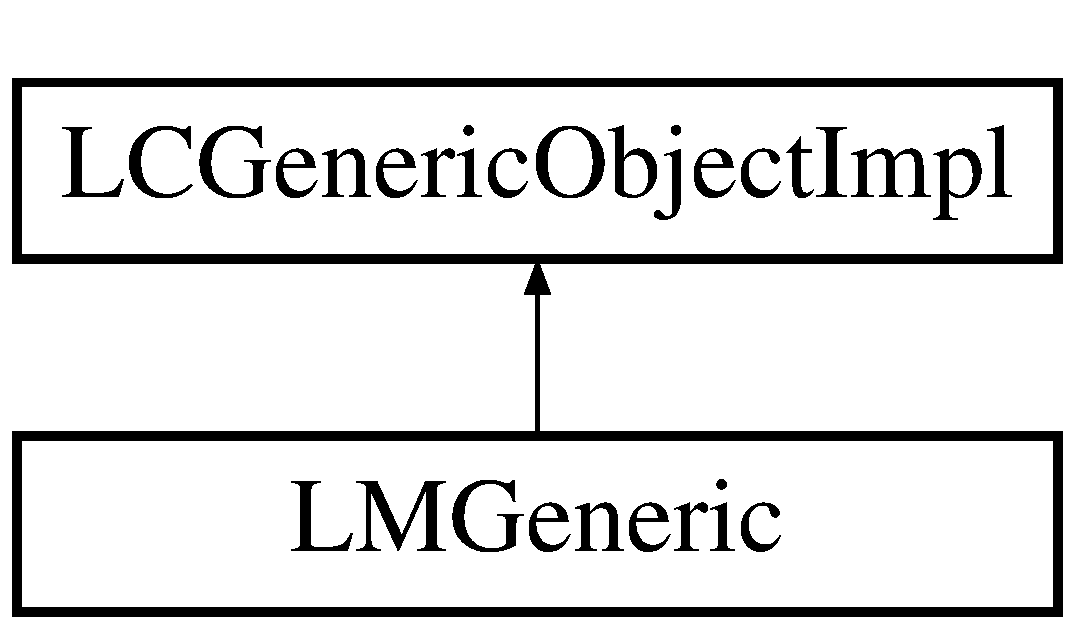
\includegraphics[height=2.000000cm]{classLMGeneric}
\end{center}
\end{figure}
\subsection*{Public Member Functions}
\begin{DoxyCompactItemize}
\item 
std\-::vector$<$ int $>$ \& {\bfseries get\-Int\-Vector} ()\label{classLMGeneric_a0f55d4095ddbe5bce59fb8b2e37ec96a}

\item 
int $\ast$ {\bfseries get\-Int\-Buffer} ()\label{classLMGeneric_aa80986fb5ac9f0d33d43f62c68a9df7f}

\item 
unsigned char $\ast$ {\bfseries get\-Char\-Buffer} ()\label{classLMGeneric_a23b9f85c15757aab82ea033ba8b69a19}

\item 
unsigned int {\bfseries n\-Bytes} ()\label{classLMGeneric_a2dfe9b4627a9c71097146060e9450795}

\item 
{\bf S\-D\-H\-C\-A\-L\-\_\-buffer} {\bfseries get\-S\-D\-H\-C\-A\-L\-Buffer} ()\label{classLMGeneric_aa89db9dad9ed04e49a9f0f6c751f8906}

\end{DoxyCompactItemize}


\subsection{Detailed Description}


Definition at line 36 of file S\-D\-H\-C\-A\-L\-\_\-\-Raw\-Data\-\_\-\-Processor.\-h.



The documentation for this class was generated from the following file\-:\begin{DoxyCompactItemize}
\item 
S\-D\-H\-C\-A\-L\-\_\-\-Raw\-Data\-\_\-\-Processor.\-h\end{DoxyCompactItemize}

\section{S\-D\-H\-C\-A\-L\-\_\-buffer Class Reference}
\label{classSDHCAL__buffer}\index{S\-D\-H\-C\-A\-L\-\_\-buffer@{S\-D\-H\-C\-A\-L\-\_\-buffer}}
Inheritance diagram for S\-D\-H\-C\-A\-L\-\_\-buffer\-:\begin{figure}[H]
\begin{center}
\leavevmode
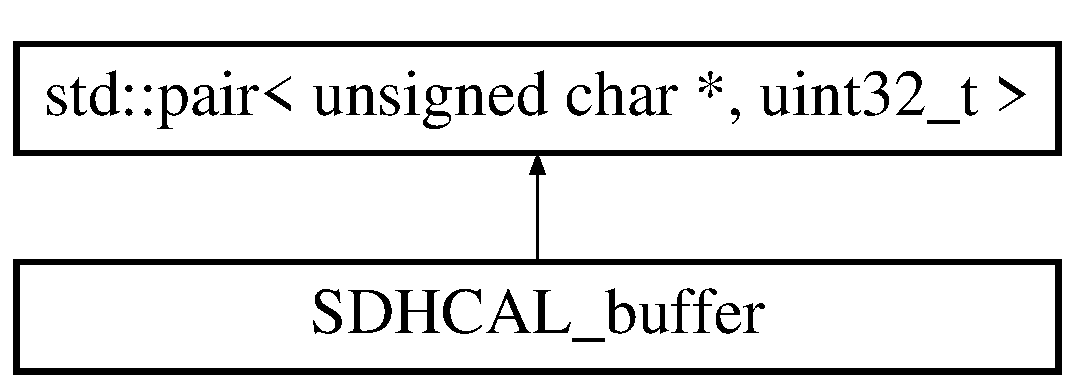
\includegraphics[height=2.000000cm]{classSDHCAL__buffer}
\end{center}
\end{figure}
\subsection*{Public Member Functions}
\begin{DoxyCompactItemize}
\item 
{\bfseries S\-D\-H\-C\-A\-L\-\_\-buffer} (unsigned char $\ast$b, uint32\-\_\-t i)\label{classSDHCAL__buffer_a66035b5c40a02dd9ff13b7f8b6f02220}

\item 
unsigned char $\ast$ {\bfseries buffer} ()\label{classSDHCAL__buffer_a62944e38a31adc9c946f7850853eccce}

\item 
unsigned char $\ast$ {\bfseries end\-Of\-Buffer} ()\label{classSDHCAL__buffer_adc6469aa1a4370f5a79c4d0440a5fa3f}

\item 
uint32\-\_\-t {\bfseries getsize} ()\label{classSDHCAL__buffer_a164f52f488dd2e7a75ab162ec7910c6e}

\item 
void {\bfseries print\-Buffer} (uint32\-\_\-t start, uint32\-\_\-t stop, std\-::ostream \&flux=std\-::cout)\label{classSDHCAL__buffer_ab8eb79883e3aa5f2428721b074fac450}

\item 
void {\bfseries print\-Buffer} (uint32\-\_\-t start=0, std\-::ostream \&flux=std\-::cout)\label{classSDHCAL__buffer_a3521819be02bb8c672271ad657c54082}

\end{DoxyCompactItemize}


\subsection{Detailed Description}


Definition at line 23 of file S\-D\-H\-C\-A\-L\-\_\-\-Raw\-Data\-\_\-\-Processor.\-h.



The documentation for this class was generated from the following file\-:\begin{DoxyCompactItemize}
\item 
S\-D\-H\-C\-A\-L\-\_\-\-Raw\-Data\-\_\-\-Processor.\-h\end{DoxyCompactItemize}

\section{S\-D\-H\-C\-A\-L\-\_\-\-Raw\-Buffer\-\_\-\-Navigator Class Reference}
\label{classSDHCAL__RawBuffer__Navigator}\index{S\-D\-H\-C\-A\-L\-\_\-\-Raw\-Buffer\-\_\-\-Navigator@{S\-D\-H\-C\-A\-L\-\_\-\-Raw\-Buffer\-\_\-\-Navigator}}
\subsection*{Public Member Functions}
\begin{DoxyCompactItemize}
\item 
{\bfseries S\-D\-H\-C\-A\-L\-\_\-\-Raw\-Buffer\-\_\-\-Navigator} ({\bf S\-D\-H\-C\-A\-L\-\_\-buffer} b)\label{classSDHCAL__RawBuffer__Navigator_a8116fb4c68067c7ecdfa3c9ad2de09cb}

\item 
bool {\bfseries valid\-Buffer} ()\label{classSDHCAL__RawBuffer__Navigator_af04cd664647277f7209475d939777cc4}

\item 
uint32\-\_\-t {\bfseries get\-Start\-Of\-D\-I\-F} ()\label{classSDHCAL__RawBuffer__Navigator_ac3f6143d2ec2cdf440b47ca6433251f1}

\item 
unsigned char $\ast$ {\bfseries get\-D\-I\-F\-Buffer\-Start} ()\label{classSDHCAL__RawBuffer__Navigator_a94dccfc4aac0d19eb20130a61d675e73}

\item 
uint32\-\_\-t {\bfseries get\-D\-I\-F\-Buffer\-Size} ()\label{classSDHCAL__RawBuffer__Navigator_a97bd22be6f726446cea9b3d141a36991}

\item 
{\bf S\-D\-H\-C\-A\-L\-\_\-buffer} {\bfseries get\-D\-I\-F\-Buffer} ()\label{classSDHCAL__RawBuffer__Navigator_a8b286baaaefc3a457e5c34457e8dccc2}

\item 
{\bf D\-I\-F\-Ptr} $\ast$ {\bfseries get\-D\-I\-F\-Ptr} ()\label{classSDHCAL__RawBuffer__Navigator_a40b03138306707a590f9fdf327d191c5}

\item 
uint32\-\_\-t {\bfseries get\-End\-Of\-D\-I\-F\-Data} ()\label{classSDHCAL__RawBuffer__Navigator_a3a220bfca852bd6ac038bfff69fa6765}

\item 
uint32\-\_\-t {\bfseries get\-Size\-After\-D\-I\-F\-Ptr} ()\label{classSDHCAL__RawBuffer__Navigator_a535452ee375e56a475ae52a4ffc1dcb9}

\item 
uint32\-\_\-t {\bfseries get\-D\-I\-F\-\_\-\-C\-R\-C} ()\label{classSDHCAL__RawBuffer__Navigator_ad85f281c4cd8205179b6b0639eb36f21}

\item 
bool {\bfseries has\-Slow\-Control\-Data} ()\label{classSDHCAL__RawBuffer__Navigator_a3fa2456e044884b3f30b894a28210065}

\item 
{\bf S\-D\-H\-C\-A\-L\-\_\-buffer} {\bfseries get\-S\-C\-Buffer} ()\label{classSDHCAL__RawBuffer__Navigator_adce9a434b3626a15646254b38b3004a9}

\item 
bool {\bfseries bad\-S\-C\-Data} ()\label{classSDHCAL__RawBuffer__Navigator_af39905619e2c3f989ad51a3a58c096fa}

\item 
{\bf S\-D\-H\-C\-A\-L\-\_\-buffer} {\bfseries get\-End\-Of\-All\-Data} ()\label{classSDHCAL__RawBuffer__Navigator_aef4e7e1e81e73588507c10bdc3c918a4}

\end{DoxyCompactItemize}


\subsection{Detailed Description}


Definition at line 50 of file S\-D\-H\-C\-A\-L\-\_\-\-Raw\-Data\-\_\-\-Processor.\-h.



The documentation for this class was generated from the following files\-:\begin{DoxyCompactItemize}
\item 
S\-D\-H\-C\-A\-L\-\_\-\-Raw\-Data\-\_\-\-Processor.\-h\item 
S\-D\-H\-C\-A\-L\-\_\-\-Raw\-Data\-\_\-\-Processor.\-cc\end{DoxyCompactItemize}

\section{S\-D\-H\-C\-A\-L\-\_\-\-Raw\-Data\-\_\-\-Processor Class Reference}
\label{classSDHCAL__RawData__Processor}\index{S\-D\-H\-C\-A\-L\-\_\-\-Raw\-Data\-\_\-\-Processor@{S\-D\-H\-C\-A\-L\-\_\-\-Raw\-Data\-\_\-\-Processor}}
Inheritance diagram for S\-D\-H\-C\-A\-L\-\_\-\-Raw\-Data\-\_\-\-Processor\-:\begin{figure}[H]
\begin{center}
\leavevmode
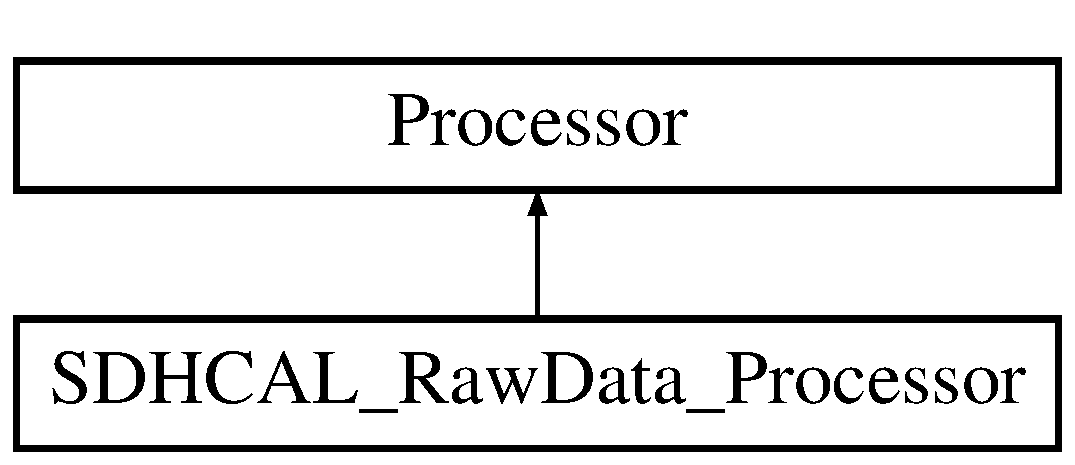
\includegraphics[height=2.000000cm]{classSDHCAL__RawData__Processor}
\end{center}
\end{figure}
\subsection*{Public Member Functions}
\begin{DoxyCompactItemize}
\item 
virtual Processor $\ast$ {\bfseries new\-Processor} ()\label{classSDHCAL__RawData__Processor_a2858a41a6e319c7421ae5a7c4bb72ce8}

\item 
virtual void {\bf init} ()
\begin{DoxyCompactList}\small\item\em Called at the begin of the job before anything is read. \end{DoxyCompactList}\item 
virtual void {\bf process\-Run\-Header} (L\-C\-Run\-Header $\ast$run)\label{classSDHCAL__RawData__Processor_a5055e1d2a481b4521389857b8e635e47}

\begin{DoxyCompactList}\small\item\em Called for every run. \end{DoxyCompactList}\item 
virtual void {\bf process\-Event} (L\-C\-Event $\ast$evt)\label{classSDHCAL__RawData__Processor_a206997e22828eff5fcb029448533e3b4}

\begin{DoxyCompactList}\small\item\em Called for every event -\/ the working horse. \end{DoxyCompactList}\item 
virtual void {\bfseries check} (L\-C\-Event $\ast$evt)\label{classSDHCAL__RawData__Processor_ab884e4f49c7cf3b10e9a68cf977cd7b3}

\item 
virtual void {\bf end} ()\label{classSDHCAL__RawData__Processor_a5ce1f6c5628449ad3ea9e4aeb0f8457b}

\begin{DoxyCompactList}\small\item\em Called after data processing for clean up. \end{DoxyCompactList}\end{DoxyCompactItemize}


\subsection{Detailed Description}


Definition at line 82 of file S\-D\-H\-C\-A\-L\-\_\-\-Raw\-Data\-\_\-\-Processor.\-h.



\subsection{Member Function Documentation}
\index{S\-D\-H\-C\-A\-L\-\_\-\-Raw\-Data\-\_\-\-Processor@{S\-D\-H\-C\-A\-L\-\_\-\-Raw\-Data\-\_\-\-Processor}!init@{init}}
\index{init@{init}!SDHCAL_RawData_Processor@{S\-D\-H\-C\-A\-L\-\_\-\-Raw\-Data\-\_\-\-Processor}}
\subsubsection[{init}]{\setlength{\rightskip}{0pt plus 5cm}void S\-D\-H\-C\-A\-L\-\_\-\-Raw\-Data\-\_\-\-Processor\-::init (
\begin{DoxyParamCaption}
{}
\end{DoxyParamCaption}
)\hspace{0.3cm}{\ttfamily [virtual]}}\label{classSDHCAL__RawData__Processor_a9e3e8e999a811d44c391d6eb5d195b86}


Called at the begin of the job before anything is read. 

Use to initialize the processor, e.\-g. book histograms. 

Definition at line 152 of file S\-D\-H\-C\-A\-L\-\_\-\-Raw\-Data\-\_\-\-Processor.\-cc.


\begin{DoxyCode}
152                                     \{ 
153 
154   \textcolor{comment}{//streamlog\_out(DEBUG) << "   init called  " << std::endl ;}
155 
156   \textcolor{comment}{// usually a good idea to}
157   printParameters() ;
158 
159 
160 \}
\end{DoxyCode}


The documentation for this class was generated from the following files\-:\begin{DoxyCompactItemize}
\item 
S\-D\-H\-C\-A\-L\-\_\-\-Raw\-Data\-\_\-\-Processor.\-h\item 
S\-D\-H\-C\-A\-L\-\_\-\-Raw\-Data\-\_\-\-Processor.\-cc\end{DoxyCompactItemize}

\section{Trivent\-Proc Class Reference}
\label{classTriventProc}\index{Trivent\-Proc@{Trivent\-Proc}}
Inheritance diagram for Trivent\-Proc\-:\begin{figure}[H]
\begin{center}
\leavevmode
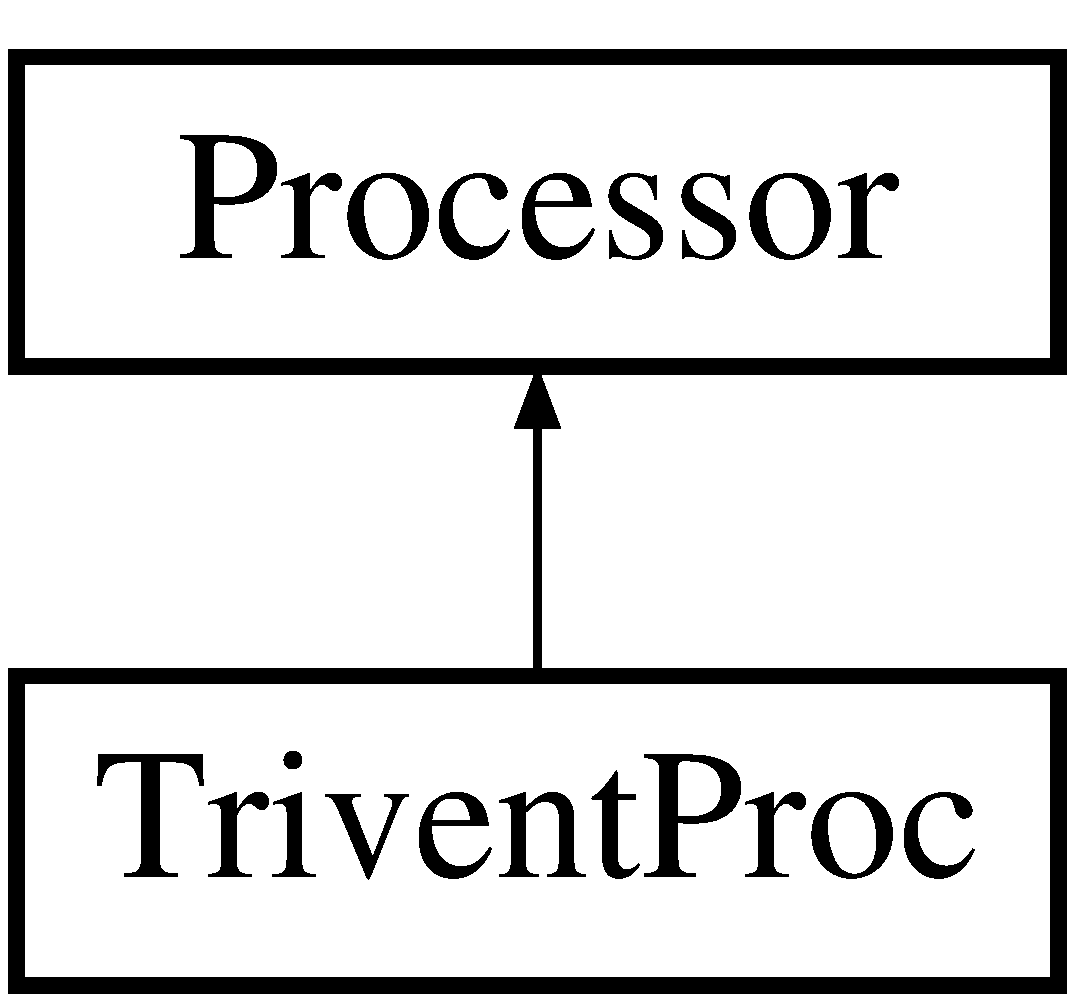
\includegraphics[height=2.000000cm]{classTriventProc}
\end{center}
\end{figure}
\subsection*{Public Member Functions}
\begin{DoxyCompactItemize}
\item 
Processor $\ast$ {\bfseries new\-Processor} ()\label{classTriventProc_a2eed3578f54694abc42fa4307dee1d20}

\item 
void {\bfseries init} ()\label{classTriventProc_ae13d0d62abd79b6836fe8eb897ee64c2}

\item 
void {\bf process\-Event} (L\-C\-Event $\ast$evt\-P)
\item 
void {\bfseries process\-Run\-Header} (L\-C\-Run\-Header $\ast$run\-H)\label{classTriventProc_a2a2ab0532cce0a212604ee07b777042d}

\item 
bool {\bfseries Min\-On\-Layer\-Cut} (int nch\-\_\-cut)\label{classTriventProc_ad0bda688a420336ce0b8eb2a1aae1534}

\item 
void {\bfseries X\-M\-L\-Reader} (std\-::string xmlfile)\label{classTriventProc_abbb736b698e72d3df8f7f3a30f280c78}

\item 
void {\bfseries read\-Dif\-Geom\-File} (std\-::string geomfile)\label{classTriventProc_a0b10dd2335c26feeefbc3f0dfd0de6c3}

\item 
void {\bfseries print\-Dif\-Geom} ()\label{classTriventProc_af2fc3368fa8ff09d0e6472fd6e0ca4a2}

\item 
uint {\bfseries get\-Cell\-Dif\-\_\-id} (int cell\-\_\-id)\label{classTriventProc_acf38b8e2ac310cdf8012089acf12dda2}

\item 
uint {\bfseries get\-Cell\-Asic\-\_\-id} (int cell\-\_\-id)\label{classTriventProc_a1fab13fc22554bfcee80d2bbc6e77510}

\item 
uint {\bfseries get\-Cell\-Chan\-\_\-id} (int cell\-\_\-id)\label{classTriventProc_af5fd540819042b9426b6c2c7485fb572}

\item 
void {\bfseries get\-Max\-Time} ()\label{classTriventProc_a42cd3e93ef2b88ead1bd2395945ea5e3}

\item 
uint\-Vec {\bfseries get\-Time\-Spectrum} ()\label{classTriventProc_a8d0b6dc0fad10f71100f617b1c970f48}

\item 
uint $\ast$ {\bfseries get\-Pad\-Index} (uint dif\-\_\-id, uint asic\-\_\-id, uint chan\-\_\-id)\label{classTriventProc_a5c8cc7cacb9b8bce67a4ca63e27afa53}

\item 
void {\bfseries event\-Builder} (L\-C\-Collection $\ast$col\-\_\-event, uint time\-\_\-peak, uint prev\-\_\-time\-\_\-peak)\label{classTriventProc_a780ee8e577ab2b70de6d416bd648b78d}

\item 
bool {\bfseries peak\-Or\-Not} (uint\-Vec time\-\_\-spectrum, uint itime, uint threshold)\label{classTriventProc_a9416baadb33709d4ae1249d25f65ff69}

\item 
void {\bfseries end} ()\label{classTriventProc_a0e407d5f7aa553911600c06a63e0de32}

\end{DoxyCompactItemize}
\subsection*{Protected Attributes}
\begin{DoxyCompactItemize}
\item 
T\-H1\-F $\ast$ {\bfseries noise\-\_\-dist}\label{classTriventProc_ac0a9072e3f7369a69a1279cd40742f5f}

\item 
T\-H1\-F $\ast$ {\bfseries gain\-\_\-chan}\label{classTriventProc_aec0086ff9d72ce4571ea717a951d7873}

\item 
T\-H1\-F $\ast$ {\bfseries mean\-\_\-hit\-\_\-dif}\label{classTriventProc_aa75d69847dd3dd9e46792239878b2bed}

\item 
T\-H1\-F $\ast$ {\bfseries time\-\_\-hit\-\_\-dif}\label{classTriventProc_a63e59016e4f099828dd6535439455548}

\item 
std\-::map$<$ std\-::string, \\*
std\-::string $>$ {\bfseries m\-\_\-parameters}\label{classTriventProc_a3514acac042237306ea8a869f38f7e68}

\item 
std\-::vector\\*
$<$ E\-V\-E\-N\-T\-::\-Raw\-Calorimeter\-Hit $\ast$ $>$ {\bfseries \-\_\-trigger\-\_\-raw\-\_\-hit}\label{classTriventProc_ab9d06de26636a08ead56e78aaa87e7a0}

\item 
bool {\bfseries G\-A\-I\-N\-\_\-\-C\-O\-R\-R\-E\-C\-T\-I\-O\-N\-\_\-\-M\-O\-D\-E}\label{classTriventProc_ac84895c8a6be617eb3332ab7a8ac37fe}

\item 
std\-::string {\bfseries \-\_\-out\-File\-Name}\label{classTriventProc_a387e40bdcac189c40e175e06815f02a5}

\item 
std\-::string {\bfseries \-\_\-noise\-File\-Name}\label{classTriventProc_a220762aa6135a107cee1ad913dad4a6d}

\item 
std\-::string {\bfseries \-\_\-tree\-Name}\label{classTriventProc_a769b399f40c85ccdeefb11e240a04524}

\item 
std\-::string {\bfseries \-\_\-logroot\-Name}\label{classTriventProc_a121c5cbee7cb958ed21c1a13d149b63f}

\item 
std\-::string {\bfseries \-\_\-col\-Name}\label{classTriventProc_adc5e858360c5d2ad5af169c5c626f914}

\item 
std\-::string {\bfseries \-\_\-file\-Name}\label{classTriventProc_a325f306ec60bc31a5d24e26ab6a4fddb}

\item 
std\-::string {\bfseries \-\_\-mappingfile}\label{classTriventProc_a989b747a0e4e6cfa02d1161a98de421b}

\item 
std\-::string {\bfseries \-\_\-geom\-X\-M\-L}\label{classTriventProc_a7c495692c2aad61a7ce60c749c5bf189}

\item 
std\-::ostream $\ast$ {\bfseries \-\_\-output}\label{classTriventProc_ad38fdb66f027efd6eaac8b638d35f85f}

\item 
std\-::vector$<$ std\-::string $>$ {\bfseries \-\_\-hcal\-Collections}\label{classTriventProc_a741619ec3d58ddd1a9744e9f57ffcb9d}

\item 
int {\bfseries \-\_\-overwrite}\label{classTriventProc_a9d01cd1a1fb76477953a190cc1c96fe8}

\item 
T\-Tree $\ast$ {\bfseries \-\_\-output\-Tree}\label{classTriventProc_ad4554751214a304dec1b09c55fd028d8}

\item 
unsigned int {\bfseries \-\_\-event\-Nr}\label{classTriventProc_afc0951084c600f51cd378430e8b1ed7f}

\item 
Int\-\_\-t {\bfseries \-\_\-\-Nhit}\label{classTriventProc_a6f03092ba886655fe7e6ef2faa6ec522}

\item 
Int\-\_\-t {\bfseries \-\_\-elec\-\_\-noise\-\_\-cut}\label{classTriventProc_a488e31f6481f5681c5286f4ad6bff084}

\item 
std\-::map$<$ int, {\bf Layer\-I\-D} $>$ {\bfseries \-\_\-mapping}\label{classTriventProc_ae9b9a0dd8dbec52b074660676aec5c3a}

\item 
std\-::map$<$ int, double $>$ {\bfseries \-\_\-chamber\-\_\-pos}\label{classTriventProc_a7976ae7b1b03e3b7b7d123d28e52b2c6}

\item 
int {\bfseries \-\_\-noise\-Cut}\label{classTriventProc_a0a1cbdfe614612719c1dd5304e2a60c4}

\item 
int {\bfseries \-\_\-time\-Win}\label{classTriventProc_a7026a2ba0c1c61fbfb14402dc933dfdc}

\item 
int {\bfseries \-\_\-\-Layer\-Cut}\label{classTriventProc_ad24c6960d10afbcef0ed02cfc7e365c7}

\item 
int {\bfseries \-\_\-time2prev\-\_\-event\-\_\-cut}\label{classTriventProc_ab300480569003a54edd34c46a63f9df4}

\item 
double {\bfseries \-\_\-layer\-\_\-gap}\label{classTriventProc_ac507176dcf02b0a8db304160ce93d63f}

\item 
float {\bfseries \-\_\-beam\-Energy}\label{classTriventProc_a1ae26de8044b04d845295bdb6ea00ae7}

\item 
int {\bfseries trig\-\_\-count}\label{classTriventProc_a77891bb090308eb5d8b57cacf06ab3c0}

\item 
int {\bfseries \-\_\-maxtime}\label{classTriventProc_aeb72fee6e655dd84b6c2142b6562ec44}

\item 
int {\bfseries evtnum}\label{classTriventProc_a7cd0658f8c4162a4b2039df7fde4c2d8}

\item 
int {\bfseries \-\_\-rejected\-Num}\label{classTriventProc_ae62a20b0357ddf5d24f6de3f9c2dd51c}

\item 
uint {\bfseries \-\_\-index} [3]\label{classTriventProc_a2966485d1996f86059e87d7b3ff419c9}

\item 
uint\-Vec {\bfseries zcut}\label{classTriventProc_ab77125d891b8f57baca23c74afdf40be}

\item 
L\-C\-Writer $\ast$ {\bfseries \-\_\-lc\-Writer}\label{classTriventProc_a5e80a938f23a70dc9a95f65903f04701}

\item 
std\-::string {\bfseries normal}\label{classTriventProc_af85b2772af2664fa71473108a7dc6bd7}

\item 
std\-::string {\bfseries red}\label{classTriventProc_ade637760722fa4dc9c4b36a2ce529027}

\item 
std\-::string {\bfseries green}\label{classTriventProc_a13a6d20c018fbf3ff83b28e5c8d3cbb4}

\item 
std\-::string {\bfseries yellow}\label{classTriventProc_a6659601453b91c2db5437e431e39ddd7}

\item 
std\-::string {\bfseries blue}\label{classTriventProc_af12ed889606a5daae796500684995b8c}

\item 
std\-::string {\bfseries magenta}\label{classTriventProc_a9a5ee47f38a27a4c8cfbeb8c1922cda8}

\item 
std\-::string {\bfseries white}\label{classTriventProc_a4a6754865dbcaadd651aaf674d5e0134}

\end{DoxyCompactItemize}


\subsection{Detailed Description}


Definition at line 27 of file Trivent\-Proc.\-hh.



\subsection{Member Function Documentation}
\index{Trivent\-Proc@{Trivent\-Proc}!process\-Event@{process\-Event}}
\index{process\-Event@{process\-Event}!TriventProc@{Trivent\-Proc}}
\subsubsection[{process\-Event}]{\setlength{\rightskip}{0pt plus 5cm}void Trivent\-Proc\-::process\-Event (
\begin{DoxyParamCaption}
\item[{L\-C\-Event $\ast$}]{evt\-P}
\end{DoxyParamCaption}
)}\label{classTriventProc_ad2327afd289a47a0a86b59f01561795c}
loop over collection

Find the condidate event 

Definition at line 518 of file Trivent\-Proc.\-cc.


\begin{DoxyCode}
519 \{       
520   \textcolor{keywordflow}{if} (evtP != NULL)\{
521     \textcolor{keywordflow}{try}\{
522       
523       \_eventNr=evtP->getEventNumber();
524       \textcolor{keywordflow}{for}(\textcolor{keywordtype}{unsigned} \textcolor{keywordtype}{int} i=0; i< \_hcalCollections.size(); i++)\{
525         \textcolor{keywordflow}{try}\{
526           
527           LCCollection * col = NULL;
528           col = evtP ->getCollection(\_hcalCollections[i].c\_str());
529           \textcolor{keywordtype}{int} numElements = col->getNumberOfElements();\textcolor{comment}{// hit number }
530           
531           
532           std::cout << yellow << \textcolor{stringliteral}{"Trigger name == "} << trig\_count++ << normal << std::endl;
533           
534           \textcolor{keywordflow}{if}(col == NULL )  \{
535             std::cout<< red << \textcolor{stringliteral}{"TRIGGER SKIPED ..."}<< normal <<std::endl;
536             \textcolor{keywordflow}{break};
537           \}
538           
539           \textcolor{keywordflow}{if}(numElements > \_elec\_noise\_cut)  \{
540             std::cout << red << \textcolor{stringliteral}{"TRIGGER SKIPED ..."}<< normal <<std::endl;
541             \textcolor{keywordflow}{break};
542           \}
543           
544           \textcolor{comment}{// set raw hits }
545           \_trigger\_raw\_hit.clear();
546           \textcolor{keywordflow}{for} (\textcolor{keywordtype}{int} ihit(0); ihit < col->getNumberOfElements(); ++ihit) \{\textcolor{comment}{// loop over the hits}
547             RawCalorimeterHit *raw\_hit = 
548               \textcolor{keyword}{dynamic\_cast<}RawCalorimeterHit*\textcolor{keyword}{>}( col->getElementAt(ihit)) ;
549             \textcolor{keywordflow}{if} (NULL != raw\_hit)\{
550               \_trigger\_raw\_hit.push\_back(raw\_hit);
551             \}
552           \}
553           getMaxTime();
554           uintVec time\_spectrum = getTimeSpectrum();
555           
556           \textcolor{comment}{//---------------------------------------------------------------}
558 \textcolor{comment}{}          uint ibin=0;
559           \textcolor{keywordtype}{double} bin\_c\_prev = -2 * \_timeWin; \textcolor{comment}{//  the previous bin center}
560           
561           \textcolor{keywordtype}{int} time\_prev = 0;
562           \textcolor{keywordflow}{while}(ibin < (\_maxtime+1))\{ 
563             \textcolor{keywordflow}{if}(time\_spectrum[ibin] >= \_noiseCut
564                && time\_spectrum[ibin] >  time\_spectrum[ibin+1]  
565                && time\_spectrum[ibin] >= time\_spectrum[ibin+1])\{
566               LCEventImpl*  evt = \textcolor{keyword}{new} LCEventImpl() ;     \textcolor{comment}{// create the event}
567               
568               \textcolor{comment}{//---------- set event paramters ------}
569               \textcolor{keyword}{const} std::string parname\_trigger = \textcolor{stringliteral}{"trigger"};
570               \textcolor{keyword}{const} std::string parname\_energy  = \textcolor{stringliteral}{"beamEnergy"};
571               evt->parameters().setValue(parname\_trigger,evtP->getEventNumber()); 
572               evt->parameters().setValue(parname\_energy , \_beamEnergy); 
573               evt->setRunNumber( evtP->getRunNumber()) ;
574               \textcolor{comment}{//-------------------------------------}
575               
576               LCCollectionVec* outcol = \textcolor{keyword}{new} LCCollectionVec(LCIO::CALORIMETERHIT);
577               TriventProc::eventBuilder(outcol,ibin,bin\_c\_prev);
578               
579               \textcolor{keywordtype}{bool} TestEvent = MinOnLayerCut(\_LayerCut);
580               \textcolor{keywordflow}{if}(TestEvent &&                                  \textcolor{comment}{// the min layer numb cut       }
581                  abs(\textcolor{keywordtype}{int}(ibin)-time\_prev) > \_time2prev\_event\_cut)\{ \textcolor{comment}{// time2prev event  cut }
582 \textcolor{preprocessor}{#if true                }
583 \textcolor{preprocessor}{}                std::cout<<green<<\textcolor{stringliteral}{" Trivent find event at :==> "}<< red << ibin 
584                          <<green<<\textcolor{stringliteral}{"\(\backslash\)t :Nhit: ==> "}<< magenta
585                          <<outcol->getNumberOfElements() << normal <<std::endl;  
586 \textcolor{preprocessor}{#endif }
587 \textcolor{preprocessor}{}                
588                 
589                 evt->setEventNumber( evtnum++ ) ;
590                 evt->addCollection(outcol, \textcolor{stringliteral}{"SDHCAL\_HIT"});
591                 \_lcWriter->writeEvent( evt ) ;
592               \}\textcolor{keywordflow}{else}\{
593                 \_rejectedNum++;
594                 \textcolor{keyword}{delete} outcol;
595               \}
596               time\_prev = ibin;
597               \textcolor{keyword}{delete} evt; evt=NULL;
598               
599               bin\_c\_prev = ibin;
600               ibin = ibin+\_timeWin;
601             \}\textcolor{keywordflow}{else}\{ibin++;\}
602           \}
603           
604         \}\textcolor{keywordflow}{catch} (lcio::DataNotAvailableException zero) \{\}
605       \}
606     \}\textcolor{keywordflow}{catch} (lcio::DataNotAvailableException err) \{\}
607   \}
608   
609            
610 \}       
\end{DoxyCode}


The documentation for this class was generated from the following files\-:\begin{DoxyCompactItemize}
\item 
Trivent\-Proc.\-hh\item 
Trivent\-Proc.\-cc\end{DoxyCompactItemize}

\addcontentsline{toc}{part}{Index}
\printindex
\end{document}
